\section{Event-Sufficient Replay Model}

The replay model is defined over architectural transitions. The original run and replay run share the same platform profile, firmware image, and initial architectural state. Between boundary events, the RV32I core semantics are deterministic. At a boundary, replay consumes the recorded event at the same commit index and validates replay-visible observations.

An event contains a commit index, a same-index order tag, a class, and a payload. Core classes are those required to drive replay in the scoped failures: MMIO read values, MMIO write observations, interrupt entry and exit, external inputs, selected stores or branch outcomes when they influence the property, checkpoint/hash values when used, and the property-failure signature. Diagnostic PC context is useful for debugging and comparator alignment, but the model does not assert a globally smallest trace.

Figure~\ref{fig:timeline} shows the intended record/replay timeline. The recorder captures only the boundary facts needed to make the replay run take the same firmware-visible path through the target failure prefix. Overflow invalidates replay availability; it is a status bit, not a recoverable compression mode.

\begin{figure}[t]
\centering
\IfFileExists{figures/replay_flow.pdf}{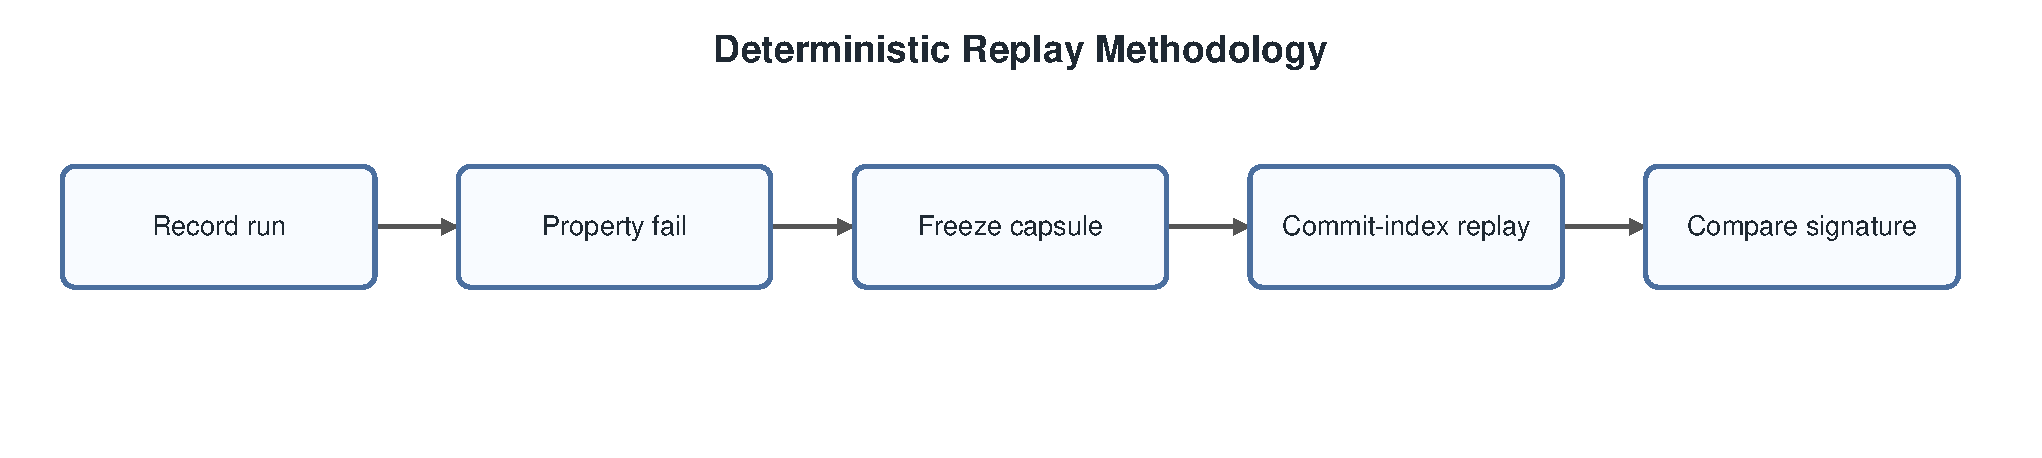
\includegraphics[width=\linewidth]{figures/replay_flow.pdf}}{\fbox{\parbox{0.9\linewidth}{Generated source: \texttt{paper/figures/replay\_flow.svg}}}}
\caption{Record/replay timeline with commit-indexed events. Source generated from \texttt{scripts/make\_figures.py}.}
\label{fig:timeline}
\end{figure}

The proof sketch in \texttt{formal/replay\_sufficiency\_theorem.md} is by induction over commit index: equal initial state, deterministic ordinary steps, equal boundary-event payloads at nondeterministic steps, and deterministic property checking over the equal prefix.
